%%%%%%%%%%%%%%%%%%%%%%%%%%%%%%%%%%%%%%%%%%%%%%%%%%%%%%%%%%%%%%%%%%%%%%%%%%%%%%%%
%2345678901234567890123456789012345678901234567890123456789012345678901234567890
%        1         2         3         4         5         6         7         8

\documentclass[letterpaper, 10 pt, conference]{ieeeconf}  % Comment this line out if you need a4paper

%\documentclass[a4paper, 10pt, conference]{ieeeconf}      % Use this line for a4 paper

\IEEEoverridecommandlockouts                              % This command is only n
\usepackage{amsfonts}
\usepackage{amsmath}
\DeclareMathOperator*{\argmax}{arg\,max}
\usepackage{graphicx}
\graphicspath{ {./figures/} }

\overrideIEEEmargins                                      % Needed to meet printer requirements.

%In case you encounter the following error:
%Error 1010 The PDF file may be corrupt (unable to open PDF file) OR
%Error 1000 An error occurred while parsing a contents stream. Unable to analyze the PDF file.
%This is a known problem with pdfLaTeX conversion filter. The file cannot be opened with acrobat reader
%Please use one of the alternatives below to circumvent this error by uncommenting one or the other
%\pdfobjcompresslevel=0
%\pdfminorversion=4

% See the \addtolength command later in the file to balance the column lengths
% on the last page of the document

% The following packages can be found on http:\\www.ctan.org
%\usepackage{graphics} % for pdf, bitmapped graphics files
%\usepackage{epsfig} % for postscript graphics files
%\usepackage{mathptmx} % assumes new font selection scheme installed
%\usepackage{times} % assumes new font selection scheme installed
%\usepackage{amsmath} % assumes amsmath package installed
%\usepackage{amssymb}  % assumes amsmath package installed
\usepackage{todonotes}
\usepackage{comment}

\title{\LARGE \bf Predicting Experienced Presence through Movement Behavior in Large Virtual Mazes}

\author{Lukas Gehrke$^{1}$, Klaus Gramann$^{1,3,4}$% <-this % stops a space
\thanks{This research was supported by a grant from the German Federal Ministry of Education and Research (01GQ1511) to KG}% <-this % stops a space
\thanks{$^{1}$Lukas Gehrke and Klaus Gramann are with Department of Biopsychology and Neuroergonomics, TU Berlin, Strasse des 17. Juni 135, 10623 Berlin, Germany
        {\tt\small lukas.gehrke@tu-berlin.de}}%
\thanks{$^{3}$Center for Advanced Neurological Engineering, University of California San Diego, USA}
\thanks{$^{4}$School of Software, University of Technology Sydney, USA}
}

\begin{document}
\maketitle
\thispagestyle{empty}
\pagestyle{empty}
%%%%%%%%%%%%%%%%%%%%%%%%%%%%%%%%%%%%%%%%%%%%%%%%%%%%%%%%%%%%%%%%%%%%%%%%%%%%%%%%

\begin{abstract}
% must be between 150 and 250, so aiming for 200!
\begin{abstract}
The use of head-mounted virtual reality (VR) to induce presence in a computer simulated world has proven to significantly increase the ecological validity of this medium. In VR, illusions of various kinds (place illusion, plausibility illusion, etc.) occur at the same time for the user to feel present. Most prominently, the embodiment illusion has proven to elicit 'realistic' behavioral as well as physiological responses, when a strong emotional stimulus such as virtual hurting of an embodied rubber hand is provided. Yet, to be able to employ VR and claim ecological validity for less emotional stimuli, the level of presence must be accounted for. We show that the level of presence impacts free spatial exploration behavior in a large scale VR navigation paradigm. Here, we investigate the impact of an established presence metric on ongoing motor behavior demonstrating an analysis framework with a high spatial resolution. We observed participants with higher presence to stay closer to the walls while exploring invisible mazes. Ultimately, we link presence to individual differences in video game experience, sex, and spatial perspective taking abilities, confirming that user characteristics are a defining part of the presence construct.
\end{abstract}
% in the end use hemingway app (http://www.hemingwayapp.com) to increase readability
% Word count is 194:
\end{abstract}

\section{Introduction}
investigate the influence of subjectively reported presence on body movements in VR

why it is interesting to look at objective predictors of presence experience. Do people that experience presence behave differently in VR? Poses questions to the ecological validity of virtual reality as an investigative tool in cognitive science with first applications in cognitive neuroscience.s


\begin{figure}[h]
\centering
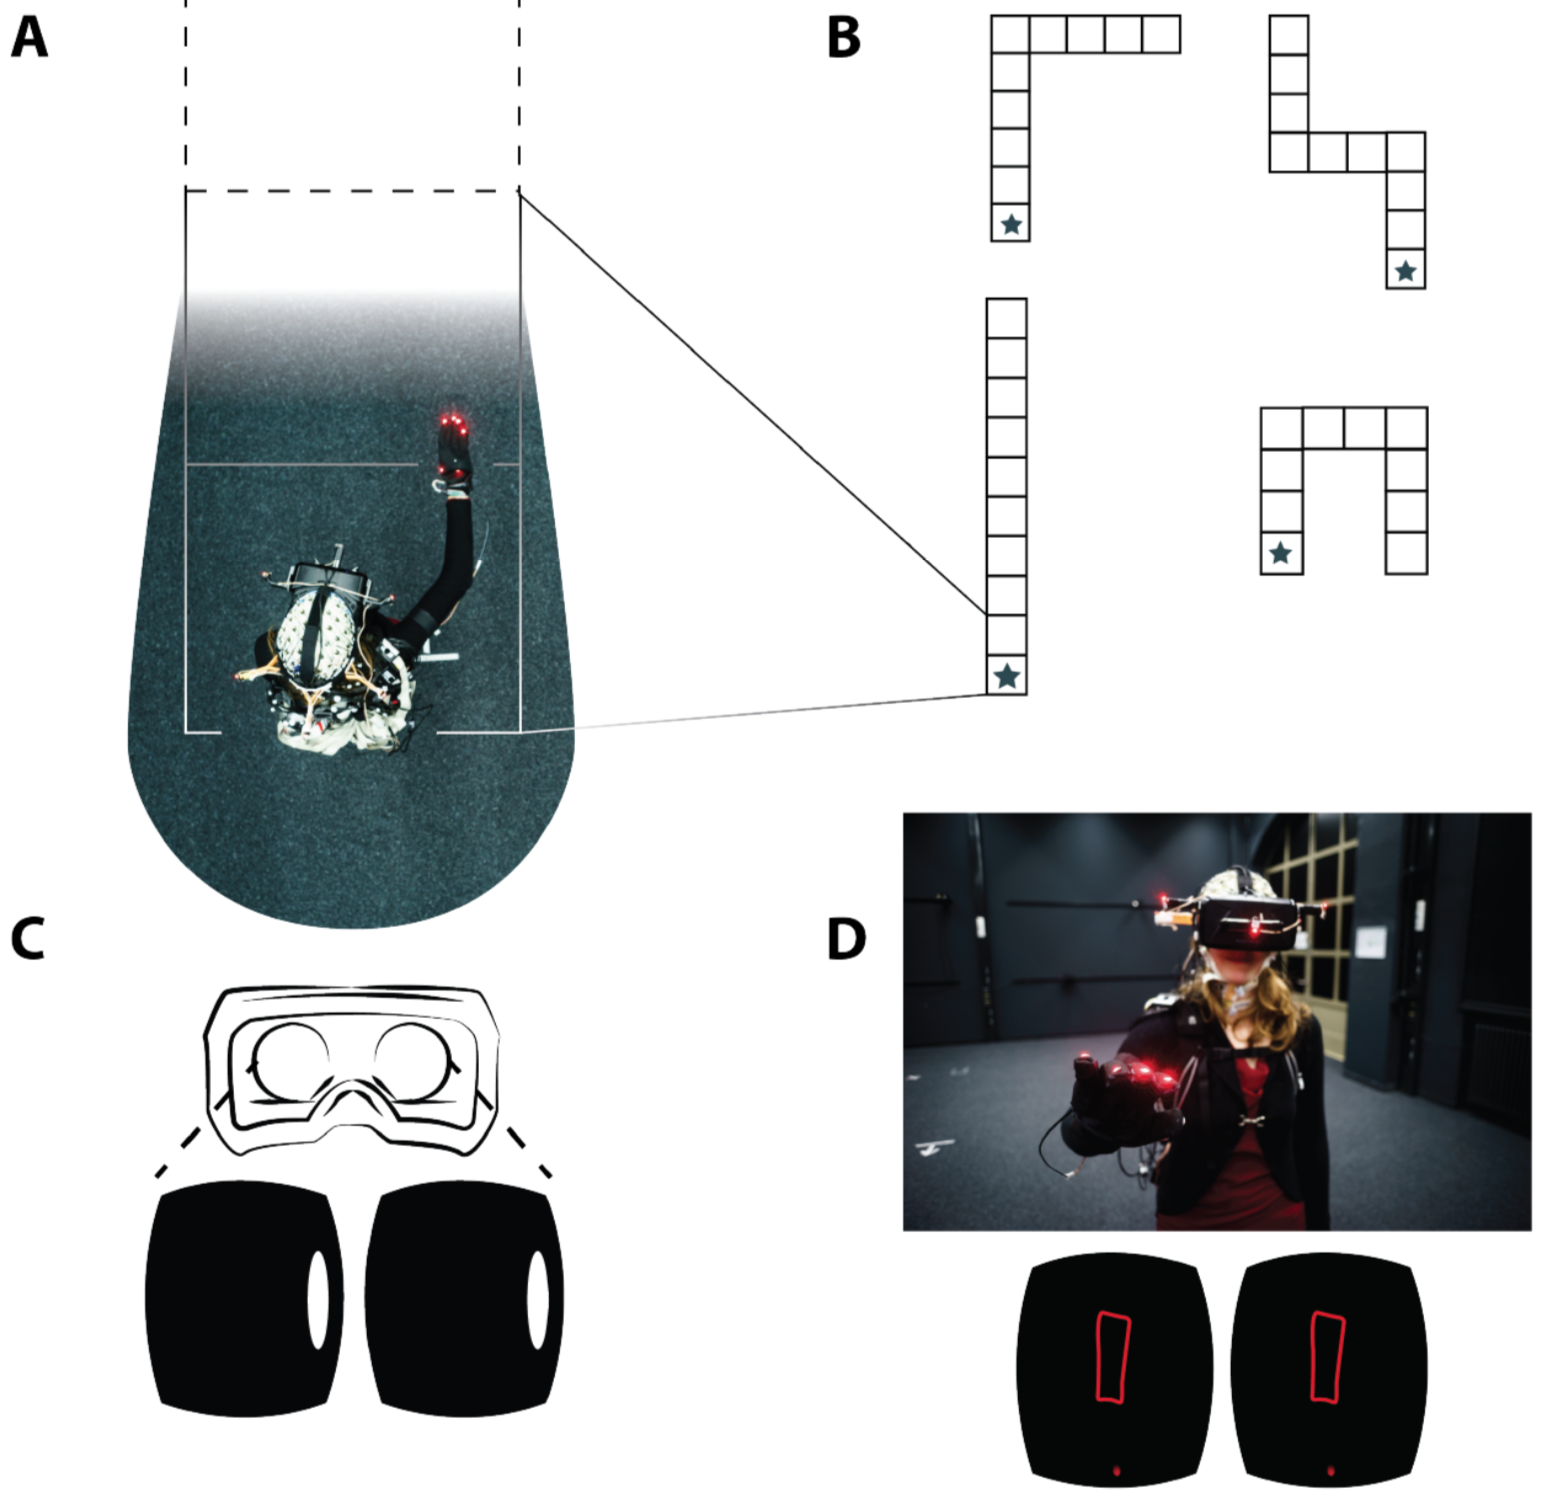
\includegraphics[width=\linewidth]{IMT_Task.png}
\vspace{0pt}
\caption{Invisible Maze Task, \textbf{A} Participant from a bird’s eye view. \textbf{B} Participants are instructed to explore four different mazes and return to the start. \textbf{C} First-person view in binocular ""VR optics"" of a wall touch. \textbf{D} Top: Participants draw a top-down view of the explored maze. Participant is equipped with 160 channels wireless EEG, head-mounted virtual reality goggles and LEDs for motion capture. Bottom: drawn sketch map. Find a detailed description in~\cite{Gehrke2018}}
\label{imt_task}
\end{figure}

\subsection{Summary and Hypotheses}
Here, we investigated the impact of experienced presence on spatial exploration behavior in the invisible maze task~\cite{Gehrke2018}. To address our motivation, we conducted the following two-step analysis. In a first step, we built a linear model to predict experienced presence given per participant descriptives. We were primarily interested to see how accurate presence can be predicted from broad knowledge of participant movement behavior. Additionally we considered a multitude of participant descriptives to derive a useful model. We reduced the model to a minimum of useful predictors so other researchers may easily reproduce our findings. In other words, we addressed how accurate subjectively reported presence may be predicted given a number of per participant descriptives.
In a second step, we increased the resolution of our analyses to specifically investigate ongoing motor behavior. Here, we analysed in detail whether participants movement behavior differed as a function of experienced presence and where it did so. To this end, we conducted mass-univariate pixel-by-pixel modeling of experienced presence on duration spent in a certain location and the number of wall touches elicited there, the simple where and what of participants actions.

% @Lukas: Should we then concentrate us on the term "place illusion" or generalize our claim to the general construct of presence? The subjective presence measure used (G1) is representing the sense of being in a place and therefore, more suitable as a metric for place illusion. If we do not want to go into much detail regarding the construct of presence, we can adapt the terminology of "the experience of presence" (also used by authors of IPQ) and in short only "presence". 

% @Sezen: no you are right, i do like place illusion much better. BTW there is a tracked changes and comment function in this overleaf now. Hit 'review' top right menu.

% @Lukas: Perfect, I tried half an hour ago without success :) Ill use from now on.

\section{Methods}
\indent \textbf{Participants.} Thirty-two healthy participants (aged 21--45 years, 14 men) took part in the
experiment. All participants gave written informed consent to participation and the experimental protocol was approved by the local ethics committee (protocol: GR\_08\_20170428). Three participants were excluded from data analysis due to incomplete data or difficulties in complying with the task requirements.

\indent \textbf{Assessing experienced presence.} In the current work, we were interested in the subjectively reported experience of presence. Therefore we analyzed the first item on 'igroup's presence questionnaire', i.e. 'In the computer generated world I had a sense of "being there"' rated from 'not at all' to 'very much'~\cite{ipq, slaterQ1}.
% The code and data are available online \todo{add link to data repository and analyses code}
\subsection{Procedure and Task}
\subsubsection{The Invisible Maze Task} Participants freely explored an interactive sparse invisible maze environment by walking and probing for virtual visual wall feedback with their hand, delivered by a virtual reality (VR) headset. Four different mazes (Fig. \ref{imt_task} B) were explored, each in three consecutive runs. Upon collision of the hand with an invisible wall, an illuminated white disc was displayed 30cm behind the collision point parallel to the invisible wall (Fig. \ref{imt_task} C). Due to the complexity of the technical details, please consult~\cite{Gehrke2018} for further details on the task, instrumentation and data collection. In summary, the task required participants to explore mazes to build a spatial representation of the maze layout. Doing the task, participants display a behavior that is comparable to explorative wall touches in the dark to find your way. We collected synchronized motion capture and behavioral events alongside high-density Electroencephalogry (EEG).
\subsection{Statistical Analyses}
\subsubsection{Predicting Presence using Participant Descriptives} First, we tested the accuracy of the predicted presence scores using general participant descriptors. We computed a least squares regression entering the IPQ presence (G1) scores as the dependent variable using R \cite{RFoundationforStatisticalComputing.2018}. For the predictors, we first computed individual averages over mazes and runs for movement velocity, exploration duration, number of wall touches, as well as sketch map accuracy. Further we added participants video game experience, sex, perspective taking and orientation ability and lastly the sense of direction into the regression model. For an explanation of each predictor see \cite{Gehrke2018}. Predictors that do not significantly add to the explanatory power of the regression model were localized using a step-wise model selection procedure based on Akaike's information criterion (AIC). The procedure was computed using 'stepAIC' of package 'MASS' \cite{Akaike1998a, Venables2002}. This procedure was selected to reduce over-fitting of the final reported model, meanwhile increasing the usability to other researchers through minimizing the number of included predictors. After the step-wise model selection, three predictors remained in the model predicting presence. Ultimately, the reduced model with three predictors was assessed in terms of its predictive accuracy. Therefore, a 5 fold cross-validation was computed to obtain a robust mean absolute error \cite{Mosteller1968, Furnkranz2011}. With 29 participants, each training fold consisted of either 23 or 24 participants with either 5 or 6 participants in the evaluated test fold. The R code and data used are available online\footnote{https://github.com/lukasgehrke/2019-IEEE-VR-Spatial-exploration-behavior-in-large-scale-VR-predicts-subjective-spatial-presence}.

\indent \textbf{Statistical Analyses II.} To enrich our analysis we strove for a greater spatial resolution of movement behavior. A general average of, e.g. movement velocity, is limited in insight due to its spatial dependence. Therefore, we constructed two-dimensional, spatial, parametric maps of the movement behavior parameters. For the different parameters, a histogram was calculated with fixed edges for each maze to be able to compare the maps across subjects. Furthermore a gaussian blur was applied to the histogram image to broaden the data and hence increase the overlap between subjects.

% Maps: heatmap head location, head velocity, wall touch location, hand jerk 2nd level: regression of presence on movement parameters, simple mcc and sig mask

\section{Results}


\subsection{Video Game Experience, Gender and Perspective Taking predict experienced Presence} Running stepwise model selection resulted in three predictors being kept, explaining 53,4\% of the variation in experienced presence ($F_{(3,25)}=11.69, p < .001,$ adjusted $R^2=.534$). Participants' predicted presence is equal to 8.15 - 1.2 (Video Game Experience) + 2.61 (SEX) - 0.02 (PTSOT) where sex is coded as 1 = Male, 2 = Female, video game experience is higher in higher scores and perspective taking ability is worse in higher scores. Video game experience ($t=-4.7, p<.001$), sex ($t=5.6, p<.001$) as well as perspective taking ability ($t=-2.52, p<.05$) were significant predictors of presence.

\subsection{Predicting Presence} Training the three predictor model above for each of five different folds of the data and evaluating its performance on the held-out fold yields a combined average .76 mean absolute error. Hence, using video game experience, sex as well as perspective taking ability we can predict experienced presence to within three-quarters of a point accuracy.
\subsection{Zooming in} add the results of the maps where duration, velocity, touches and jerk are resolved in xy.

\begin{figure}[h]
\centering
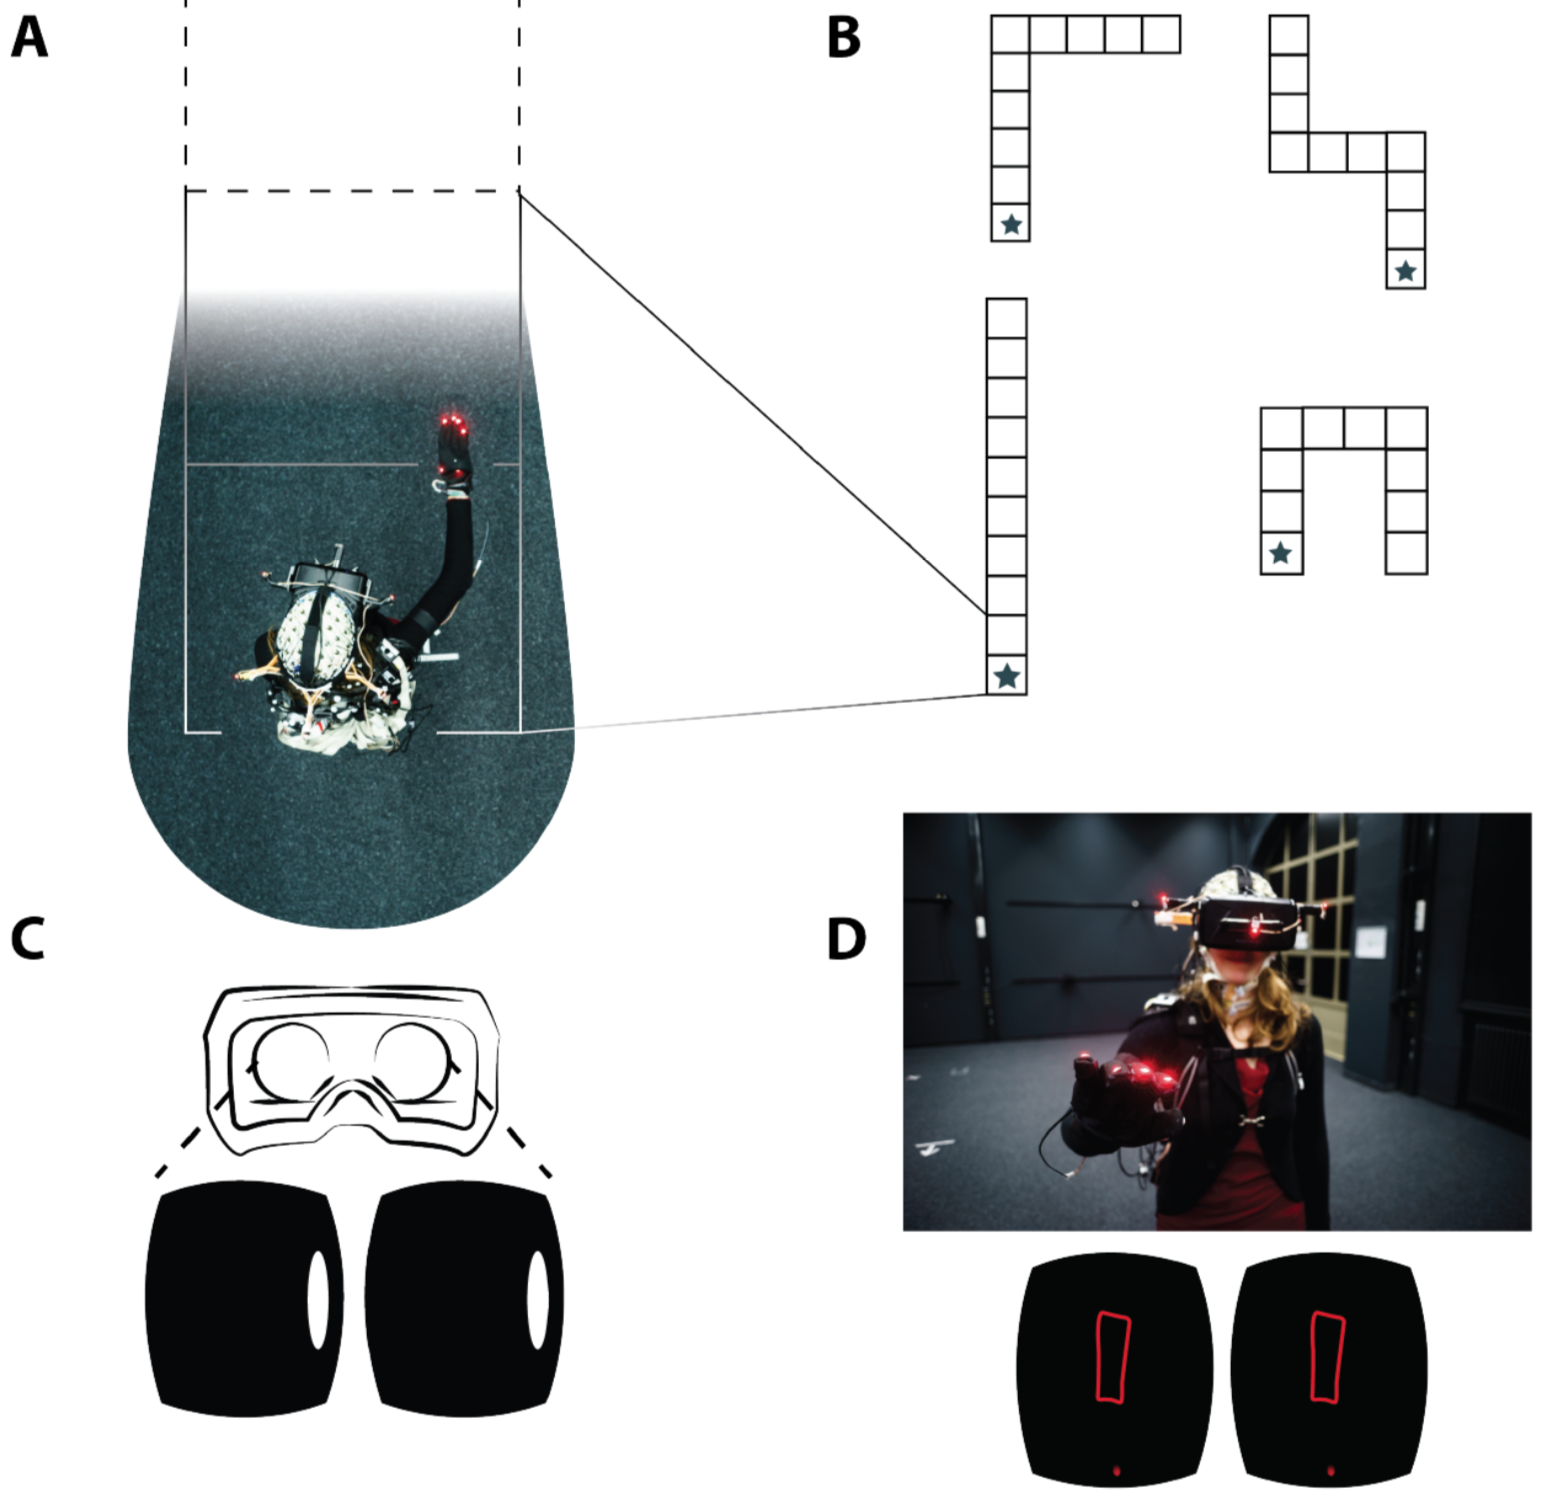
\includegraphics[width=\linewidth]{IMT_Task.png}
\vspace{0pt}
\caption{results duration mean}
\label{results_dur_mean}
\end{figure}

\begin{figure}[h]
\centering
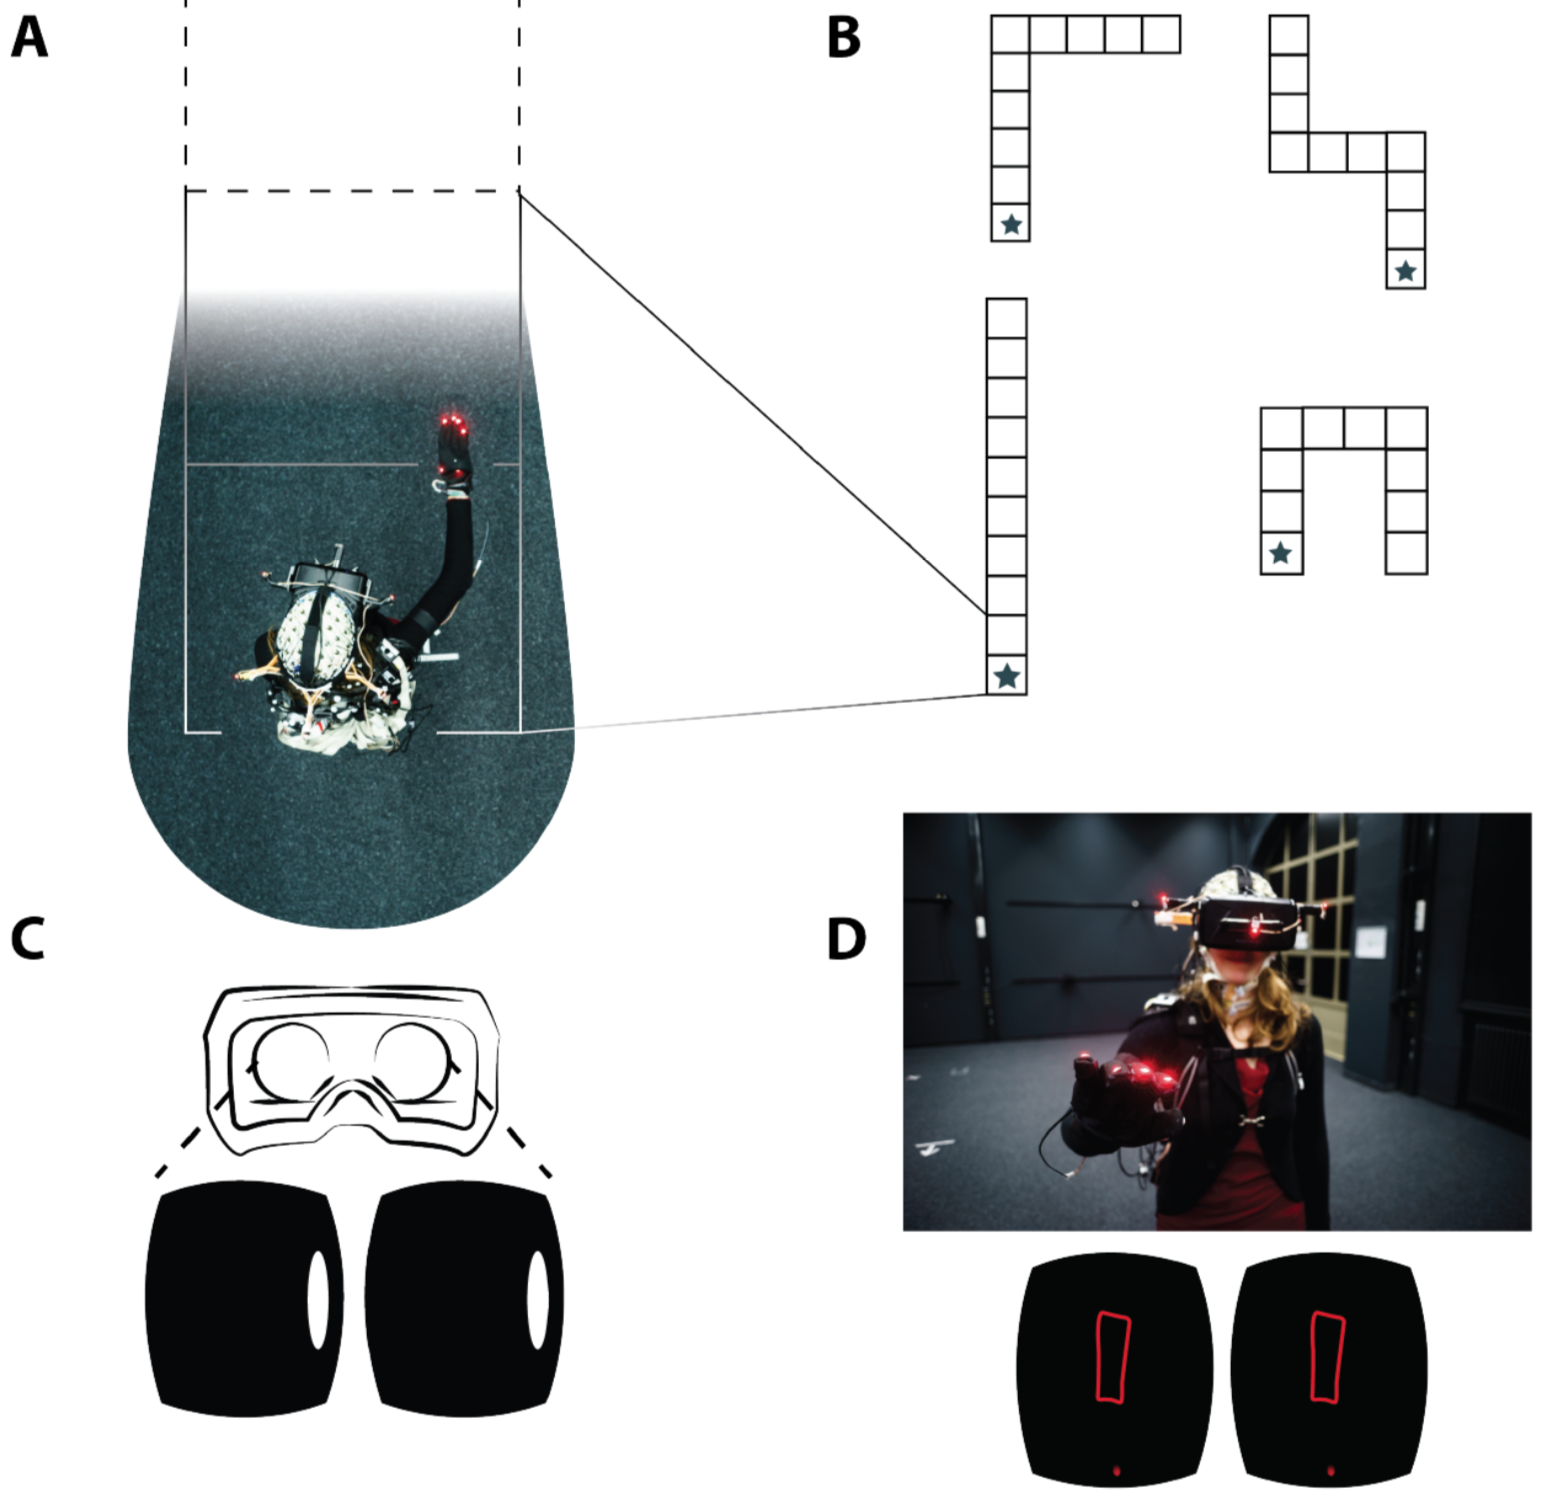
\includegraphics[width=\linewidth]{IMT_Task.png}
\vspace{0pt}
\caption{results duration and velocity}
\label{results_dur_effect}
\end{figure}

\begin{figure}[h]
\centering
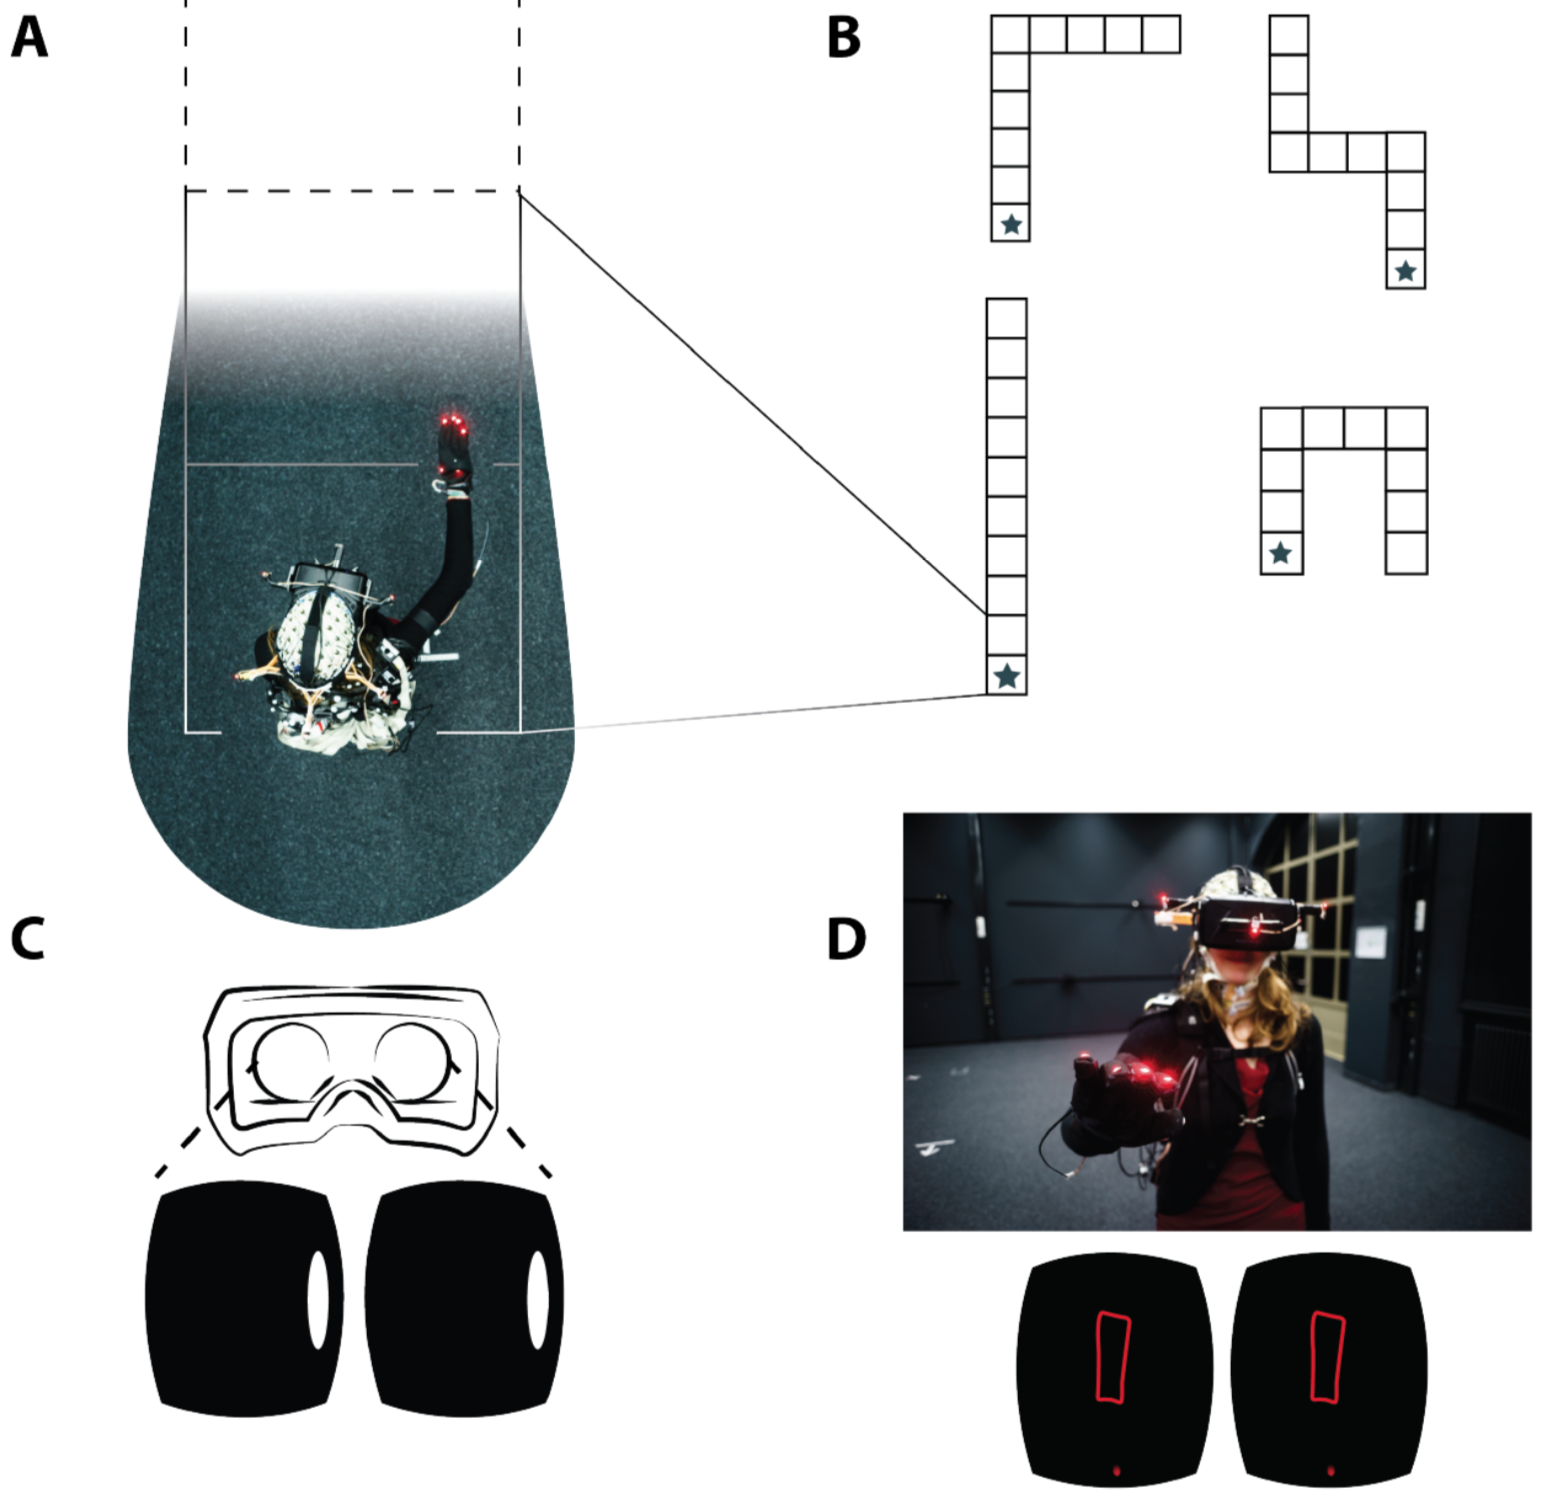
\includegraphics[width=\linewidth]{IMT_Task.png}
\vspace{0pt}
\caption{results duration and velocity}
\label{results_touches_mean}
\end{figure}

\begin{figure}[h]
\centering
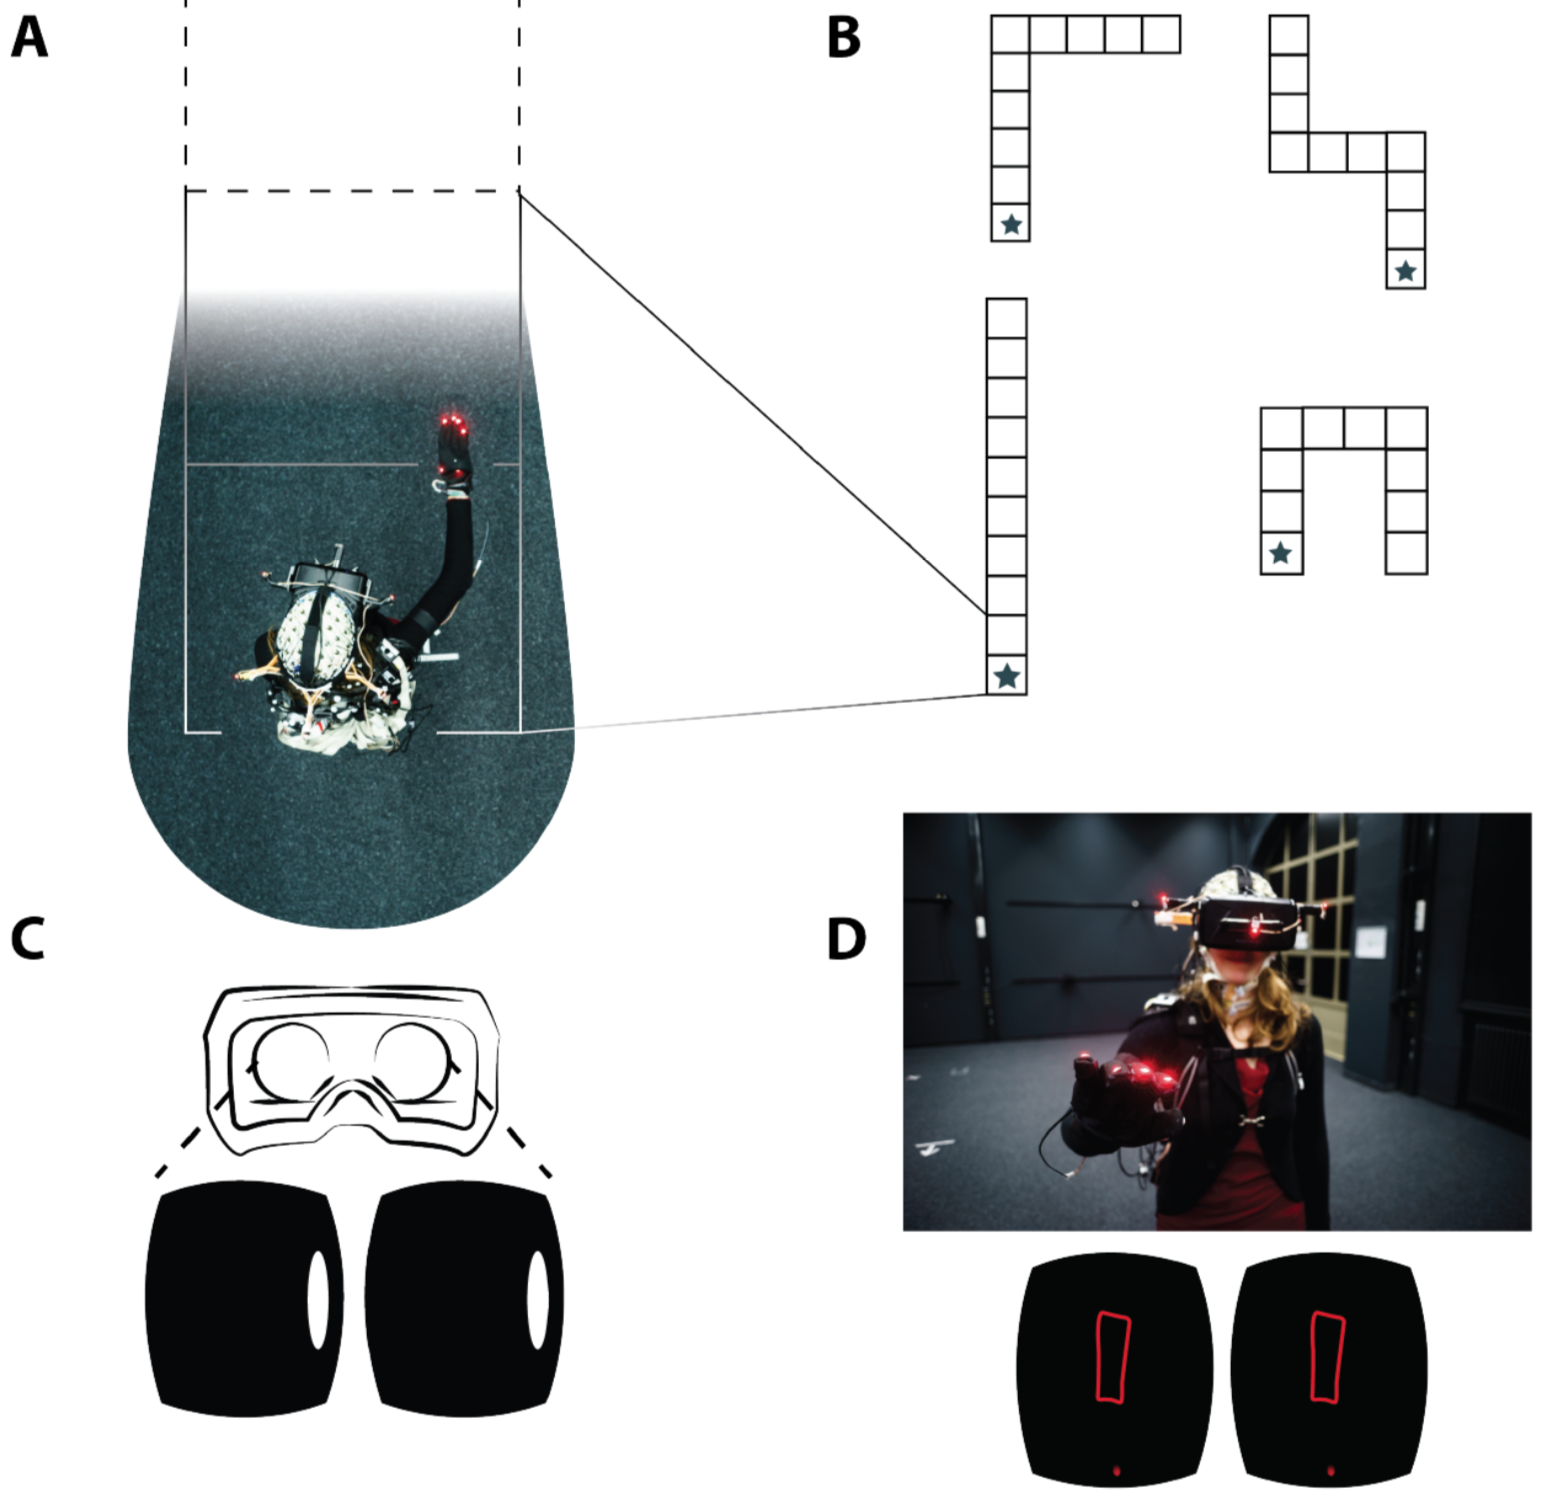
\includegraphics[width=\linewidth]{IMT_Task.png}
\vspace{0pt}
\caption{results duration and velocity}
\label{results_touches_effect}
\end{figure}

\begin{comment}

interpretation histogram binning:
how many samples fall within 1 bin -> samples/srate = duration in seconds per bin, also must consider step size when calculating

what does imagesc return after that? interpretation should stay the same and be sensible -> returns just the gaussian smoothing over the peak that is the histogram count

interpreting regression:
with an increase in presence x more seconds where spent at point xy
for easy interpretation we introduce the reasoning: participants with a higher reported presence spent 1.8 seconds longer at point (4,5 located in the outer corner of the first turn)

interpreting regression:
with an increase in presence participants moved slower closer to the wall and faster in when in the center of the maze path.

for easy interpretation we introduce the reasoning: for each 1 point increase in reported presence, participants walked x km per hour faster when at the center of the maze path and x kmh slower when getting closer to the walls.

\end{comment}

\section{Discussion}
presence and accuracy of motor behavior, problem because non-continouous metric, cite myself, moderated by learning/difficulty, clustering approaches

presence is best predicted by video game experience and sex (there is evidence of sex and videogame influence in slater work etc.). Interestingly, in our experiment video game experience negatively impacts presence reported on the general item of the IPQ. This may be due to the overly simplistic visuals of the virtual world. Participants with significant video gaming experience might perceive the world as too artificial.

explore exit interviews and use in discussion!

\indent \textbf{Disentangling Presence.}

Sense of ownership, sense of agency etc.

\indent \textbf{Outlook.}

Increasing the resolution of the investigation to finely resolved analysis in space. Motion capture allows us to do that.

% put first image of heatmaps of location and then hint at using mass-univariate regression on each point to increase the resolution of the investigative lens
say that behavioral metrics not informative enough in terms of presence with broad resolution, and that a finer resolution is beneficial.

Here, we addressed a potential link between presence and accuracy of motor behavior on broad scale, i.e. in an unconstrained navigation paradigm. 

The problem that we do assess it using non-continuous metrics with a time delay of administration~\cite{Gehrke:2019:DVM:3290605.3300657}

Complexity of presence as a psychological construct and that it may interact with spatial learning and task difficulty among other things~\cite{} % gonzales-castro model

%%%%%%%%%%%%%%%%%%%%%%%%%%%%%%%%%%%%%%%%%%%%%%%%%%%%%%%%%%%%%%%%%%%%%%%%%%%%%%%%
\addtolength{\textheight}{-12cm}   % This command serves to balance the column lengths
                                  % on the last page of the document manually. It shortens
                                  % the textheight of the last page by a suitable amount.
                                  % This command does not take effect until the next page
                                  % so it should come on the page before the last. Make
                                  % sure that you do not shorten the textheight too much.

%%%%%%%%%%%%%%%%%%%%%%%%%%%%%%%%%%%%%%%%%%%%%%%%%%%%%%%%%%%%%%%%%%%%%%%%%%%%%%%%

\input{bibliography.bib}
\end{document}